%%%% IACR Transactions TEMPLATE %%%%
% This file shows how to use the iacrtrans class to write a paper.
% Written by Gaetan Leurent gaetan.leurent@inria.fr (2020)
% Public Domain (CC0)


%%%% 1. DOCUMENTCLASS %%%%
\documentclass[journal=tosc,preprint]{iacrtrans}
%%%% NOTES:
% - Change "journal=tosc" to "journal=tches" if needed
% - Change "submission" to "final" for final version
% - Add "spthm" for LNCS-like theorems


%%%% 2. PACKAGES %%%%
\usepackage{lipsum} % Example package -- can be removed
%%%% 3. AUTHOR, INSTITUTE %%%%
\author{Ajay Tarole\inst{1} \and Ashish Kumar Suraj\inst{2} and Rudraksh Kashyap\inst{3}}
\institute{
  11840090, IIT Bhilai, \email{ajayt@iitbhilai.ac.in}
  \and
  1184230, IIT Bhilai, \email{ashishs@iitbhilai.ac.in}
  \and
  11840970, IIT Bhilai, \email{rudrakshk@iitbhilai.ac.in}
  
}
%%%% NOTES:
% - We need a city name for indexation purpose, even if it is redundant
%   (eg: University of Atlantis, Atlantis, Atlantis)
% - \inst{} can be omitted if there is a single institute,
%   or exactly one institute per author


%%%% 4. TITLE %%%%
\title{PRESENT Cipher}
%%%% NOTES:
% - If the title is too long, or includes special macro, please
%   provide a "running title" as optional argument: \title[Short]{Long}
% - You can provide an optional subtitle with \subtitle.

\begin{document}

\maketitle


%%%% 5. KEYWORDS %%%%
\keywords{PRESENT \and Differential cryptanalysis \and Linear Cryptanalysis}


%%%% 6. ABSTRACT %%%%
\begin{abstract}
  In this paper we describe the design of the PRESENT cipher and comment on the design decisions taken while developing the cipher. We also discuss Differential cryptanalysis and Linear
  cryptanalysis on round reduced version of the Cipher. 
\end{abstract}


%%%% 7. PAPER CONTENT %%%%
\section{Introduction}
As we know Advanced Encryption Standard(AES) and Data Encryption Standard (DES) are the most
studied algorithms in cryptanalysis and both algorithms have proven resistance against various cryptanalysis techniques developed
to compromise the security of ciphers. The Present cipher is a lightweight cipher designed with the goal of hardware
performance on low powered devices while providing reasonable security. The structure of the Present is distinctly similar to AES. Similar to AES the round
reduced versions are vulnerable to various cryptanalysis techniques including Linear and
Differential cryptanalysis. The Present
cipher is now ISO/IEC 29192-2:2019 standard. The cipher is majorly used in applications
with low computing power like RFID cards or IoT nodes. 
\section{List of contributions}
\begin{enumerate}
	\item Rudraksh Kashyap: Rudraksh analysed the design choices of the PRESENT cipher. He examined the properties of the S-box and the permutation layar. He studied and analysed the specifications of the cipher and he also implemented the cipher in C. 
	\item Ajay Tarole : Ajay analyed differential cryptanalysis and also implemented the differential attack on the 3-rounds of the PRESENT cipher in C using the idea of differential and filtering.
	\item Ashish Kumar Suraj : Ashish analysed the Linear properties and Integral propetries of the PRESENT cipher. He also analysed the resistance of the cipher against linear attacks. 
	
\end{enumerate}
\section{The Present Cipher}
The PRESENT cipher has a block length of 64 bits and it supports 80-bit and 128-bit keys. We describe and analyze the 80-bit key version of Present cipher as security provided by an 80-bit keys is adequate for applications like RFID tags and IoT security. The present cipher has a public S-box, Bit Permutation, and key schedule. The cipher is an Ultra-Lightweight block cipher.\\\\
The PRESENT cipher has a public S-box, Bit Permutation, and key schedule.
\subsection{Substitution-Permutation Network}
\begin{figure}[H]
	\centering
	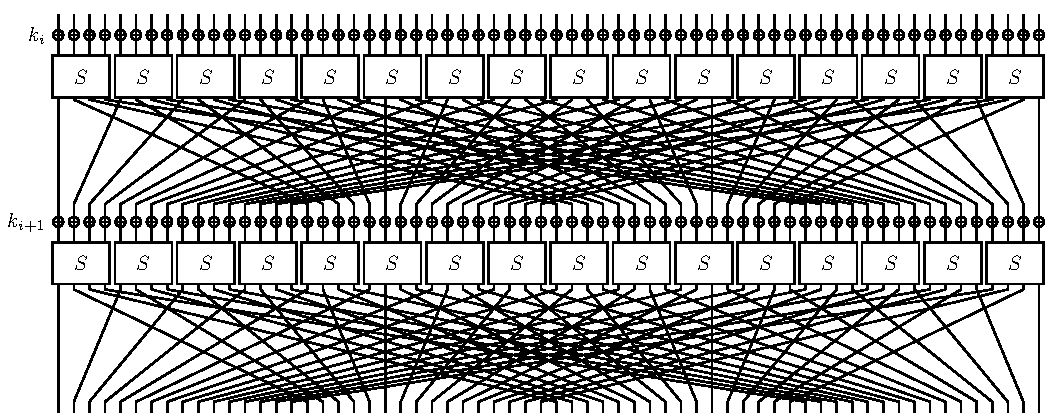
\includegraphics[width=\linewidth]{PRESENT_diagram.pdf}
	\caption{SP Network for PRESENT Cipher}
\end{figure}
\subsection{Cipher Design}
The Present-80 is an example of SP-network. Figure.2 shows the higher level pseudo-code for implementing the encryption
algorithm. The PRESENT cipher has 31 rounds and each round consists of a the round key followed by 4-bit non-linear substitution layer and linear bit-wise
permutation. The 4-bit S-Box is applied 16 times for the 64-bit input during
each round. 
\begin{figure}[h!]
	\centering
	\includegraphics[width=0.34\linewidth, height=0.15\textheight]{"Screenshot from 2021-11-06 08-28-01"}
	\caption{Pseudo Code for PRESENT cipher encryptiom}
	\label{fig:screenshot-from-2021-11-06-08-28-01}
\end{figure}\\

\subsection{Add Round Key}
Provided the round key $K_i = k_{63},k_{62} \dots k_0$ for $1\leq i \leq 32$ and the current state $S = s_{63},s_{62}\dots s_0$, addRoundKey performs the following operation\\
\hspace*{30mm}$
	S \xrightarrow{} S \oplus K_i \\
\hspace*{20mm}	\implies s_t \xrightarrow[]{} s_t \oplus k_t 
$\\
for $0\leq t\leq 63$.
\subsection{Substitution Layer}
\begin{table}[h!]
\caption{Present sBox}
\centering
\begin{tabular}{ |c||c|c|c|c|c|c|c|c|c|c|c|c|c|c|c|c| }
		\hline
		$x$ & 0 & 1 & 2 & 3&4& 5& 6&7&8&9&A&B&C&D&E&F  \\ \hline
		$S[x]$& C & 5 & 6& B &9 &0 &A &D& 3& E &F& 8& 4 &7& 1& 2 \\ \hline
\end{tabular}
\end{table}
The S-box is 4-bit to 4-bit mapping. The S-box is a mapping $S:F_2^4 \rightarrow F_2^4$ where F is a finite field. Table 1 shows the mapping of S-Box in
 Hexadecimal notation.
\\\\
To improve the avalanche-effect, the PRESENT S-Box satisfies the following conditions.\\
\begin{enumerate}
	\item For any fixed input difference $\Delta_I \in \mathbb{F}_2^4,\Delta_I \not = 0$ and output difference $\Delta_O \in \mathbb{F}_2^4,\Delta_I \not = 0$, the following condition must be satisfied
	\begin{equation*}
	\#\{ x \in \mathbb{F}_2^4~~ \vert~~ S(\Delta_I +x) + S(x) = \Delta_O \}| \leq 4
	\end{equation*}
	\item For any fixed input difference $\Delta_I \in \mathbb{F}_2^4,\Delta_I \not = 0$ and output difference $\Delta_O \in \mathbb{F}_2^4$ such that $wt(\Delta_O) = wt(\Delta_I) = 1$, the following condition must be satisfied
	\begin{equation*}
	\{ x \in \mathbb{F}_2^4~~ \vert~~  S(\Delta_I +x) + S(x) = \Delta_O  \} = \Phi
	\end{equation*}
	where $wt(x)$ is the hamming weight of $x$.
\end{enumerate}
\subsection{Permutation Layer}
The permutation layer is a bit permutation. The permutation function P(i) maps the $i^{th}$ bit of input to P(i) in the output of the permutation layer. The Table 2 is the mapping of P(i) in tabular form.
\begin{table}[h!]
	\caption{pLayer}
	\centering
	\begin{tabular}{ |c||c|c|c|c|c|c|c|c|c|c|c|c|c|c|c|c| }
		\hline
		i& 0 &1 &2 &3& 4& 5& 6 &7 &8 &9 &10 &11 &12 &13 &14 &15 \\
		P(i) &0& 16& 32& 48& 1& 17& 33&49& 2 &18& 34& 50& 3 &19 &35 &51 \\\hline\hline
		i &16& 17& 18& 19& 20& 21 &22& 23 &24 &25 &26 &27 &28 &29 &30 &31 \\
		P(i)& 4 &20 &36& 52& 5& 21 &37& 53& 6 &22& 38& 54& 7 &23 &39 &55 \\\hline\hline
		i &32& 33& 34& 35& 36& 37 &38& 39 &40 &41 &42 &43 &44 &45 &46 &47 \\
		P(i) &8 &24& 40& 56 &9& 25 &41 &57 &10 &26 &42 &58 &11 &27 &43 &59 \\\hline\hline
		i &48& 49& 50 &51 &52 &53& 54& 55 &56 &57 &58 &59 &60 &61 &62 &63 \\
		P(i) &12& 28& 44&60& 13 &29& 45& 61 &14 &30 &46 &62 &15 &31 &47 &63 \\\hline
	\end{tabular}
	
\end{table}
\subsection{Key schedule Algorithm}
The PRESENT cipher supports 80-bit or 128-bit long key but in this section we discuss the 80-bit key schedule algorithm. Firstly, the initial 80-bit key is stored in a key register $K$ and is represented as $K = k_{79}k_{78}$..$k_0$. At any round $i$, PRESENT extracts the 64-bits round key $K_i = \mathrm{k_{63}}\mathrm{k_{62}}$..$\mathrm{k_{0s}}$ from the current Key (left most 64 bits) register as follows : 
\begin{equation*}
K_i = \mathrm{k_{63}}\mathrm{k_{62}}..\mathrm{k_{0s}} = k_{79}k_{78}..k_{16}
\end{equation*}
After round key extraction, the key register $K$ is updated according to the following rules : 
\begin{enumerate}
	\item The contents of the key register $K$ is rotated by 61-bits to the left.
	\begin{equation*}
	[k_{79}k_{78}..k_{0}] = [k_{18}k_{17}..k_{20}k_{19}]
	\end{equation*}
	\item The 4-leftmost bits of the key register $K$ is passed through the PRESENT S-box.
	\begin{equation*}
	[k_{79}k_{78}k_{77}k_{76}] = S[k_{79}k_{78}k_{77}k_{76}]
	\end{equation*}
	\item The 5-bits of key register $k$, $k_{19}k_{18}k_{17}k_{16}k_{15}$ is exclusive-ored with the least significant bits of the round counter value $i$. 
	\begin{equation*}
	[k_{19}k_{18}k_{17}k_{16}k_{15}] = [k_{19}k_{18}k_{17}k_{16}k_{15}] \oplus round-counter
	\end{equation*}
\end{enumerate}
\section{Security Analysis/Attacks}
In this section, we present the results of security analysis of PRESENT.
\subsection{Differential cryptanalysis}
In this section, we use $X = x_{15},x_{14},...,x_{1},x_{0}$ to denote the XOR difference of the 16 nibbles in each step, where $x_0$ being the least significant nibble And we denote $K_i$ as the subkey for $i^{th}$ round. \\\\
We first, present the Difference Distribution table (DDT) of S-box in Table 3.
\begin{table}[h!]
	\caption{DDT of the S-box}
	\centering
	
	\begin{tabular}{ |c||c|c|c|c|c|c|c|c|c|c|c|c|c|c|c|c| }
		\hline
		& 0 & 1 & 2 & 3&4& 5& 6&7&8&9&A&B&C&D&E&F  \\ \hline \hline
		0& 16 & 0 & 0 & 0 &0 &0 &0 &0& 0& 0 &0& 0& 0 &0& 0& 0 \\ 
		1& 0 & 0 & 0 & 4 & 0 & 0 & 0 & 4 & 0 & 4 &0& 0& 0 &4& 0& 0 \\
		2& 0 & 0 & 0 & 2 & 0 & 4 & 2 & 0 & 0 & 0 &2& 0& 2 &2& 2& 0 \\
		3& 0 & 2 & 0 & 2 & 2 & 0 & 4 & 2 & 0 & 0 &2& 2& 0 &0& 0& 0 \\
		4& 0 & 0 & 0 & 0 & 0 & 4 & 2 & 2 & 0 & 2 &2& 0& 2 &0& 2& 0 \\
		5& 0 & 2 & 0 & 0 & 2 & 0 & 0 & 0 & 0 & 2 &2& 2& 4 &2& 0& 0 \\
		6& 0 & 0 & 2 & 0 & 0 & 0 & 2 & 0 & 2 & 0 &0& 4& 2 &0& 0& 4 \\
		7& 0 & 4 & 2 & 0 & 0 & 0 & 2 & 0 & 2 & 0 & 0 & 0 & 2 & 0 & 0 & 4\\
		
		8& 0 & 0 & 0 & 2 & 0 & 0 & 0 & 2 & 0 & 2 & 0 & 4 & 0 & 2 & 0 & 4\\
		9& 0 & 0 & 2 & 0 & 4 & 0 & 2 & 0 & 2 & 0 & 0 & 0 & 2 & 0 & 4 & 0\\
		A& 0 & 0 & 2 & 2 & 0 & 4 & 0 & 0 & 2 & 0 & 2 & 0 & 0 & 2 & 2 & 0\\
		B& 0 & 2 & 0 & 0 & 2 & 0 & 0 & 0 & 4 & 2 & 2 & 2 & 0 & 2 & 0 & 0\\
		C& 0 & 0 & 2 & 0 & 0 & 4 & 0 & 2 & 2 & 2 & 2 & 0 & 0 & 0 & 2 & 0\\
		D& 0 & 2 & 4 & 2 & 2 & 0 & 0 & 2 & 0 & 0 & 2 & 2 & 0 & 0 & 0 & 0\\
		E& 0 & 0 & 2 & 2 & 0 & 0 & 2 & 2 & 2 & 2 & 0 & 0 & 2 & 2 & 0 & 0\\
		F& 0 & 4 & 0 & 0 & 4 & 0 & 0 & 0 & 0 & 0 & 0 & 0 & 0 & 0 & 4 & 4\\ \hline
	\end{tabular}
\end{table}\\
From the properties of the S-box and permutation layer, we will now make some important observations. We divide the 16 S-box into 4 groups.\\\\
 We can observe the following properties from S-box : 
\begin{enumerate}
	\item The inputs of the S-box is come from 4 separate S-boxes of the same group. 
	\item The inputs to a group of 4 S-boxes come from 16 different S-boxes.
	\item The output from an S-box go into 4 distinct S-boxes, each of which belongs to a distinct group of S-boxes in the next round.
	\item The output of S-boxes from different group go to different S-boxes. 
\end{enumerate}
\begin{figure}[h!]
	\centering
	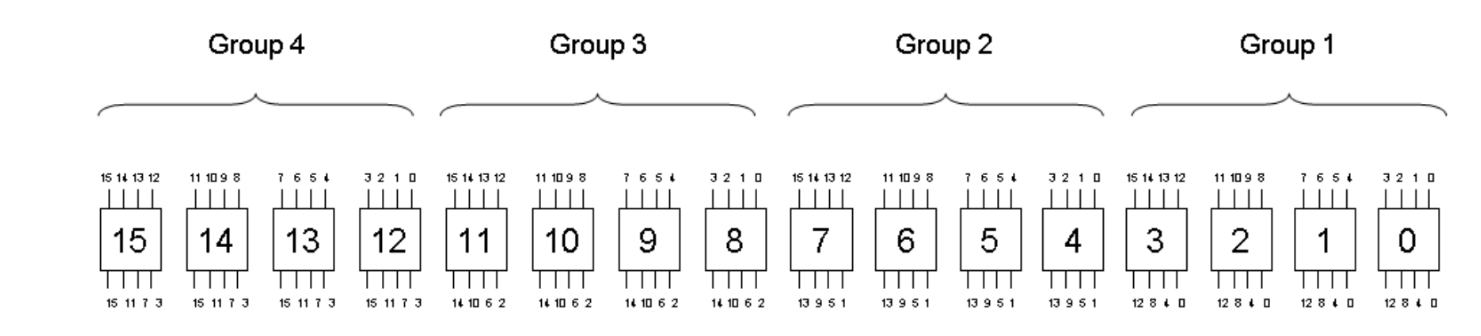
\includegraphics[width=1.0\linewidth, height=0.19\textheight]{groups}
	\caption{Groups of Sboxes}
	\label{fig:groups}
\end{figure}
Now, from the above observations(S-box properties) and the DDT, we conclude that one bit input difference will cause at least two bits output difference, resulting in at least two active S-boxes in the next round and the maximum differential probability of the DDT is $2^{-2}$. 
\subsection{Differential Characteristics}
\begin{figure}[h!]
	\centering
	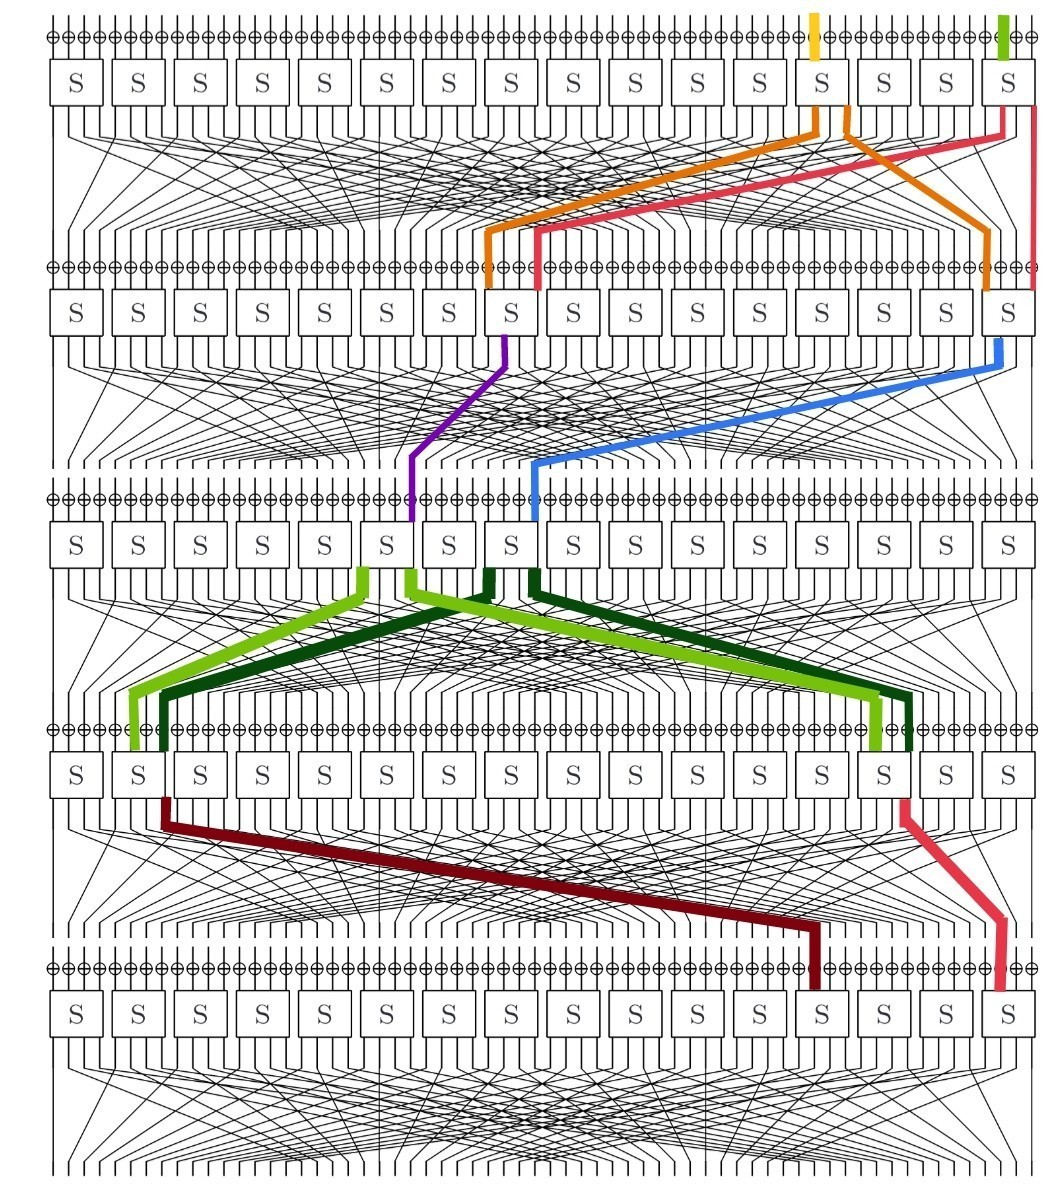
\includegraphics[width=0.72\linewidth, height=0.65\textheight]{IMG_20211114_110332}
	\caption{4-round iterative characteristics with probability $2^{-18}$}
	\label{fig:img20211114110332}
\end{figure}
\newpage
\begin{table}[h!]
	\caption{Round wise probability we have to pay}
	\centering
	\begin{tabular}{ |c||c|c|c| }
		\hline
		Rounds & & Diff. & Prob. \\ \hline \hline
		I& & $x_3 = 4$, $x_0 = 4$ &  \\ 
		$R_1$& S & $x_3 = 5$, $x_{0} = 5$ & $2^{-4}$ \\
		$R_1$& P & $x_8 = 9$, $x_{0} = 9$ & 1 \\
		$R_2$& S & $x_8 = 4$, $x_{0} = 4$ & $2^{-4}$ \\
		$R_2$& P & $x_{10} = 1$, $x_{8} = 1$ & 1 \\
		$R_3$& S & $x_{10} = 9$, $x_{8} = 9$ & $2^{-4}$ \\
		$R_3$& P & $x_{14} = 5$, $x_{2} = 5$ & 1 \\
		$R_4$& S & $x_{14} = 1$, $x_{2} = 1$  & $2^{-6}$ \\
		$R_4$& P & $x_4 = 4$, $x_0 = 4$ & 1 \\ \hline
	\end{tabular}\\
\end{table}
Here we are paying $2^{-18}$ probality and we will reach to our initial input $x_3 = 4$ and $x_0 = 4$ after 4 rounds. Now using the above diffirencial charateristics we can reach next four round(5-8) by paying another $2^{-18}$ probability. So overall we found 8 round iterative diffirencial charateristics with probability $2^{-36}$. For 12 rounds we have to pay $2^{-54}$ and for 14 round we have to pay $2^{-62}$ probability.
\begin{table}[h!]
	\centering
	\begin{tabular}{ |c||c|c|c| }
		\hline
		Rounds & & Diff. & Prob. \\ \hline \hline
		$I$&  & $x_0 = 4$, $x_{3} = 4$ &  \\
		$R_1$& S & $x_3 = 5$, $x_{0} = 5$ & $2^{-4}$ \\
		$R_1$& P & $x_8 = 9$, $x_{0} = 9$ & 1 \\
		$R_2$& S & $x_8 = 4$, $x_{0} = 4$ & $2^{-4}$ \\
		$R_2$& P & $x_{10} = 1$, $x_{8} = 1$ & 1 \\
		$R_3$& S & $x_{10} = 9$, $x_{8} = 9$ & $2^{-4}$ \\
		$R_3$& P & $x_{14} = 5$, $x_{2} = 5$ & 1 \\
		$R_4$& S & $x_{14} = 1$, $x_{2} = 1$  & $2^{-6}$ \\
		$R_4$& P & $x_4 = 4$, $x_0 = 4$ & 1 \\
		$R_5$& S & $x_3 = 5$, $x_{0} = 5$ & $2^{-4}$ \\
		$R_5$& P & $x_8 = 9$, $x_{0} = 9$ & 1 \\
		$R_6$& S & $x_8 = 4$, $x_{0} = 4$ & $2^{-4}$ \\
		$R_6$& P & $x_{10} = 1$, $x_{8} = 1$ & 1 \\
		$R_7$& S & $x_{10} = 9$, $x_{8} = 9$ & $2^{-4}$ \\
		$R_7$& P & $x_{14} = 5$, $x_{2} = 5$ & 1 \\
		$R_8$& S & $x_{14} = 1$, $x_{2} = 1$  & $2^{-6}$ \\
		$R_8$& P & $x_4 = 4$, $x_0 = 4$ & 1 \\
		$R_9$& S & $x_3 = 5$, $x_{0} = 5$ & $2^{-4}$ \\
		$R_9$& P & $x_8 = 9$, $x_{0} = 9$ & 1 \\
		$R_{10}$& S & $x_8 = 4$, $x_{0} = 4$ & $2^{-4}$ \\
		$R_{10}$& P & $x_{10} = 1$, $x_{8} = 1$ & 1 \\
		$R_{11}$& S & $x_{10} = 9$, $x_{8} = 9$ & $2^{-4}$ \\
		$R_{11}$& P & $x_{14} = 5$, $x_{2} = 5$ & 1 \\
		$R_{12}$& S & $x_{14} = 1$, $x_{2} = 1$  & $2^{-6}$ \\
		$R_{12}$& P & $x_4 = 4$, $x_0 = 4$ & 1 \\
		$R_{13}$& S & $x_3 = 5$, $x_{0} = 5$ & $2^{-4}$ \\
		$R_{13}$& P & $x_8 = 9$, $x_{0} = 9$ & 1 \\
		$R_{14}$& S & $x_8 = 4$, $x_{0} = 4$ & $2^{-4}$ \\
		$R_{14}$& P & $x_{10} = 1$, $x_{8} = 1$ & 1 \\
		\hline
	\end{tabular}
\end{table}
\subsection{Attack}
In this section, we define how exactly we attack the 3-Round Reduced PRESENT Cipher.
For this attack, we use $2^{18}$ chosen plain text pairs. Only 2 active S-boxes $(S_0 $ and $S_3)$ in the first round. Only two bit input difference in plaintext pairs at position 0th bit and 14th bit. Rest of the S-boxes are not active in the first round. \\\\
\textbf{Round Reduced Attack:}\\
\begin{figure}[h!]
	\centering
	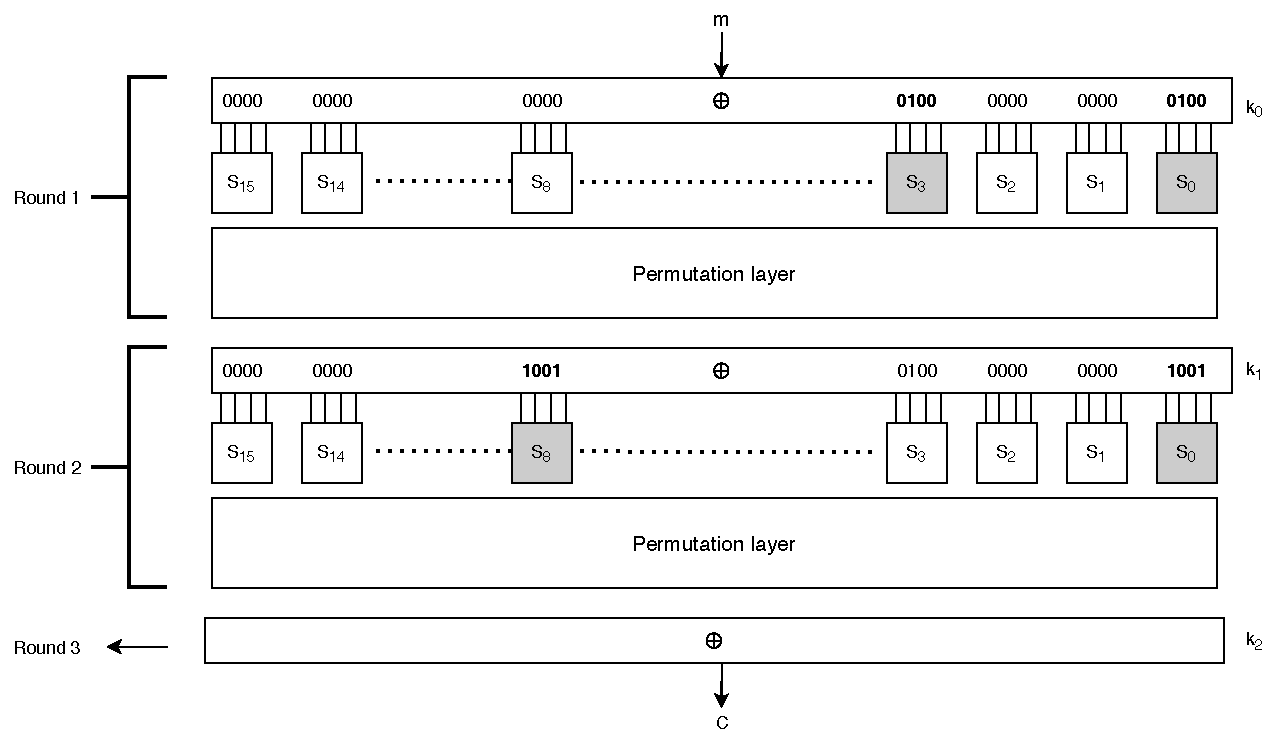
\includegraphics[width=0.9\linewidth, height=0.3\textheight]{DC1}
	\caption{Attack on 3-Round Reduced PRESENT Cipher}
	\label{fig:dc1}
\end{figure}\\
\textbf{Characteristic:}\\\\
\begin{table}[h!]
	\caption{Characteristics}
	\centering
	\begin{tabular}{ |c||c|c|c| }
		\hline
		Rounds & & Diff. & Prob. \\ \hline \hline
		I& & $x_0 = 4$, $x_4 = 4$ &  \\ 
		$R_1$& $k_0$ & $x_0 = 4$, $x_4 = 4$ & 1 \\
		$R_1$& S & $x_0 = 5$, $x_{3} = 5$ & $2^{-4}$ \\
		$R_1$& P & $x_0 = 9$, $x_{8} = 9$ & 1 \\
		$R_2$& $k_1$ & $x_0 = 9$, $x_{8} = 9$ & 1 \\ \hline
	\end{tabular}\\
\end{table}
	($x_0 = 4$, $x_3 = 4$) $\xrightarrow[]{\text{R}}$ ($x_0 = 9$, $x_8 = 9$)\\\\
\textbf{Idea of filtering:}\\
1. Decrease Wrong pair $\rightarrow$ Idea of filtering\\
2. Observe from the DDT that transitions from
	9 $\rightarrow$ {2, 4, 6, 8, c, e}\\
3. Thus, after the effect of permutation layer of the second round, $c_1 \oplus c_2$ must belong to the set given below : \\ 
$\{\{x_4=1,x_6=1\},\{x_6=1,x_8=1\},\{x_4=1,x_6=1,x_8=1\},\{x_6=1,x_{12}=1\},\{x_6=1,x_8=1,x_{12}=1\},...\}$ We have written code for this.\\\\
Note: Thus, message pair leading to the cipher text difference other than the above set, can be discarded. \\\\
So, after filtering only $2^{14}$ plaintext pairs are left in our case.\\\\
\textbf{Key Guess:}\\
\begin{figure}[h!]
	\centering
	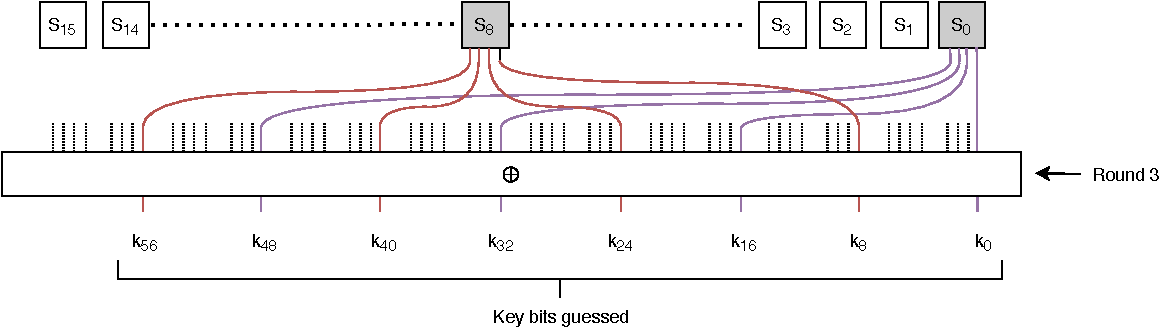
\includegraphics[width=0.9\linewidth, height=0.2\textheight]{DC2}
	\caption{Guess 8 bits of the key $k_2$}
	\label{fig:dc2}
\end{figure}\\
We are able to find 8 bits of key $k_2$. In our case only  8 bit right  subkey holds for all $2^{14}$ filtered pairs.
\subsection{Analysing the attack}
\textbf{Complexity Analysis:}\\\\
\textbf{Data:} $2^{18}$ plaintext pairs or $2^{19}$ plaintexts\\\\
\textbf{Memory:} $2^{14}$ array used to store filtered pairs\\\\
\textbf{Time:} \\\\ 
Filtering: \\
2 round encryption of $2^{18}$ plaintext pairs and compare every pairs with set of 36 possible ciphertext that we are using for filtering. \\\\
$36 \times ({2 \times 2 \times 2^{18}}) = 2^{5.17} \times 2^{20} = 2^{25.17}$\\\\
Attack:\\
2 round encryption of $2^{14}$ filtered plaintext pairs  then $2^{6}$ key gueses and $2^{14}$  ciphertext pairs decrypt for 1 round.\\\\
$2 \times (2 \times 2^{14}) + 2^6 \times (2 \times 2^{14}) = 2^{16} + 2^{21} \approx 2^{22} $\\\\
\textbf{(Data, Time, Memory)} = $(2^{19},2^{25.17},2^{14})$\\\\\\
\subsection{Linear cryptanalysis}
In this section, we will analyse the linear approximation of the PRESENT Cipher. We first present the Linear Approximation Table of PRESENT:\\
\begin{table}[h!]
	\centering
	\caption{LAT of the S-box}
	\begin{tabular}{ |c||c|c|c|c|c|c|c|c|c|c|c|c|c|c|c|c| }
		\hline
		& 0 & 1 & 2 & 3&4& 5& 6&7&8&9&A&B&C&D&E&F  \\ \hline \hline
		0& 8 & - & - & - & - & - & - & - & - & - & - & - & - & - & - & - \\ 
		1& - & - & - & - & - & -4 & - & -4 & - & - & - & - & - & -4 & - & 4 \\
		2& - & - & 2 & 2 & -2 & -2 & - & - & 2 & -2 & - & 4 & - & 4 & -2 & 2 \\
		3& - & - & 2 & 2 & 2 & -2 & -4 & - & -2 & 2 & -4 & - & - & - & -2 & -2 \\
		4& - & - & -2 & 2 & -2 & -2 & - & 4 & -2 & -2 & - & -4 & - & - & -2 & 2 \\
		5 & - & - & -2 & 2 & -2 & 2 & - & - & 2 & 2 & -4 & - & 4 & - & 2 & 2\\
		6 & - & - & - & -4 & - & - & -4 & - & - & -4 & - & - & 4 & - & - & -\\
		7 & - & - & - & 4 & 4 & - & - & - & - & -4 & - & - & - & - & 4 & -\\
		8 & - & - & 2 & -2 & - & - & -2 & 2 & -2 & 2 & - & - & -2 & 2 & 4 & 4\\
		9 & - & 4 & -2 & -2 & - & - & 2 & -2 & -2 & -2 & -4 & - & -2 & 2 & - & -\\
		A & - & - & 4 & - & 2 & 2 & 2 & -2 & - & - & - & -4 & 2 & 2 & -2 & 2\\
		B & - & -4 & - & - & -2 & -2 & 2 & -2 & -4 & - & - & - & 2 & 2 & 2 & -2\\
		C & - & - & - & - & -2 & -2 & -2 & -2 & 4 & - & - & -4 & -2 & 2 & 2 & -2\\
		D & - & 4 & 4 & - & -2 & -2 & 2 & 2 & - & - & - & - & 2 & -2 & 2 & -2\\
		E & - & - & 2 & 2 & -4 & 4 & -2 & -2 & -2 & -2 & - & - & -2 & -2 & - & -\\
		F & - & 4 & -2 & 2 & - & - & -2 & -2 & -2 & 2 & 4 & - & 2 & 2 & - & -\\
		\hline
	\end{tabular}
\end{table}\\
We observe some important properties about the LAT of the PRESENT S-box.
\begin{itemize}
	\item Maximum bias of all linear approximations $ \le 2^{-2}$
	\item Maximum linear approximation of a single bit is $\le 2^{-3}$
\end{itemize}
   We first try to bound the bias of \textbf{four} round of PRESENT using the above observations. Remember the pilling up lemma for m independent events (involving m S-boxes), according to which, the probability of linear approximation is given by :
\begin{equation*}
\frac{1}{2} + 2^{m-1} \prod_{i=1}^{m} \left( p_i  - \frac{1}{2} \right)
\end{equation*}\\
hence, the bias is given by:
\begin{equation*}
2^{m-1}\prod_{i=1}^{m} \epsilon_i
\end{equation*}
The number of active S-boxes in the four rounds can differ, and depending upon the number of active S-boxes involved, we have 3 cases to consider as below (Let the bias of 4-round of PRESENT involving i active S-boxes is denoted as $\epsilon_4^{(i)}$) : 
\begin{enumerate}
	\item Let the number of active S-boxes involved are 4, each round having one active S-box. Then, the maximum bias of the 2 active S-boxes in the middle of the rounds is atmost $2^{-3}$ and the bias of the other two rounds will be atmost $2^{-2}$, as depicted in the figure below.

    \begin{figure}[h!]
	\centering
	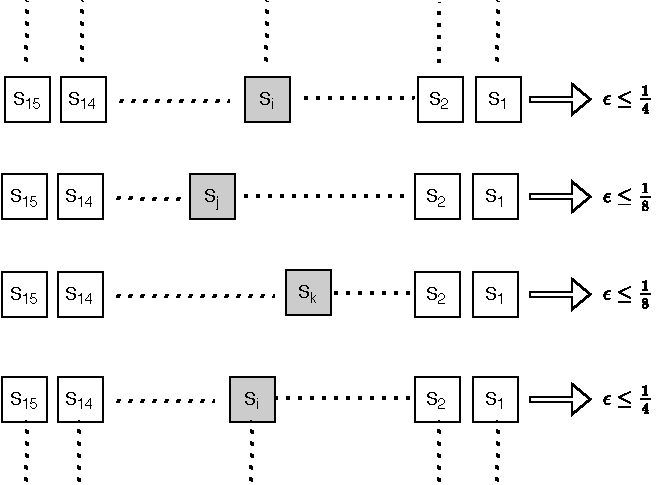
\includegraphics[width=0.7\linewidth, height=0.4\textheight]{LC}
	\caption{}
	\label{fig:lc}
    \end{figure}
Thus, the bias of this case is bounded by (using pilling up lemma): 
	\begin{equation*}
	\epsilon_4^{(4)} \leq 2^{4-1} \times (2^{-2})^2 \times (2^{-3})^2
	\end{equation*}
	\begin{equation*}
	\epsilon_4^{(4)} \leq 2^{-7} 
	\end{equation*}
	\item Let the number of S-boxes involved over the 4 rounds are 5. Then, the pattern of the active S-boxes cannot be $1-2-1-1$ or $1-1-2-1$. From the above observations, about the S-box we know that, since, the two active S-boxes are initiated by same S-box in the prev. round, therefore they must belong two different sets. Hence, they will activate at least two S-box in the next round. Therefore, the possible pattern for this case is 2-1-1-1 or 1-1-1-2 and hence the bias is bounded by : 
	\begin{equation*}
	\epsilon_4^{(5)} \leq 2^{5-1} \times (2^{-2})^4 \times (2^{-3})
	\end{equation*}
	\begin{equation*}
	\epsilon_4^{(5)} \leq 2^{-7} 
	\end{equation*}
	\item Let the number of active S-boxes is more than 5. In this case, the maximum bias for each round is $\frac{1}{4}$. Therefore, we have : 
	\begin{equation*}
	\epsilon_4^{(i)} \leq 2^{i-1} \times (2^{-2})^i \;\; for \;\; i > 5
	\end{equation*}
	Clearly, the bias is equal to $2^{-7}$ for $i = 6$ and for $i > 6$, the bias is strictly less that $2^{-7}$. 
\end{enumerate}
Thus, from the above analysis, we can conclude that the bias of 4-rounds of linear approximation of present is bounded by $2^{-7}$, that is, $\epsilon_4 \leq 2^{-7}$. Now, we can use this result to bound the linear approximation bias for 28 rounds of PRESENT, which is :
\begin{equation*}
\epsilon_{28} \leq 2^{6} \times \epsilon_4^{7} = 2^6 \times (2^{-7})^7 \implies \epsilon_{28} \leq 2^{-43}
\end{equation*}
Even for single bit recovery, a good estimate for the number of known plain-texts (N) required for a successful attack is given by : $N = c|\epsilon|^{-2}$, where constant $c \geq 2$. Thus, to attack 31 rounds of PRESENT, the attacker will have to approximate 28 rounds of PRESENT, which will require an order of $2^{86}$ known plain-texts. This, even exceeds the available space which is $2^{64}$.\\\\
\textbf{Two round characteristics:}
\begin{figure}[h!]
	\centering
	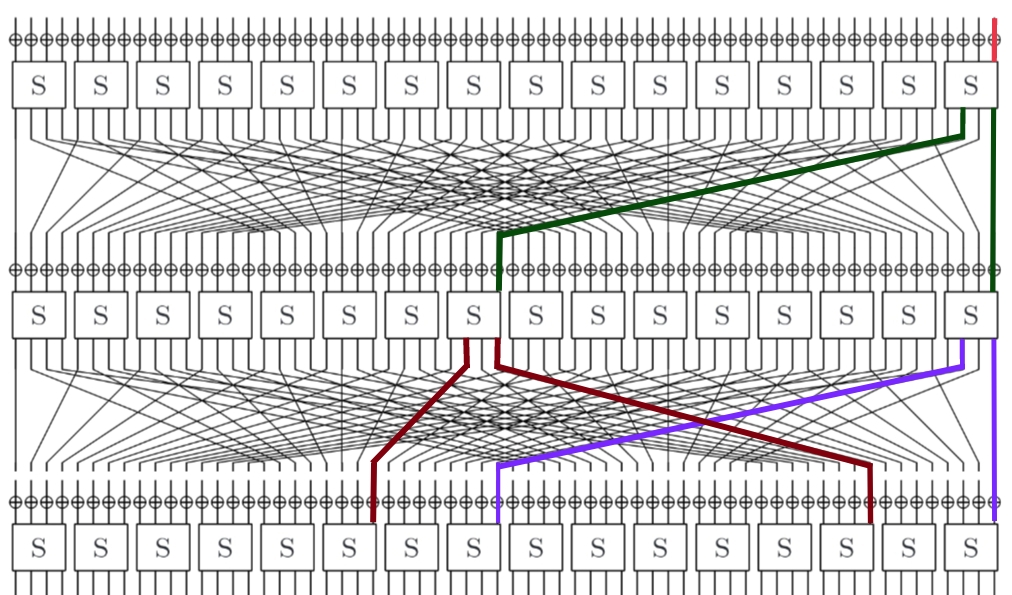
\includegraphics[width=1.0\linewidth, height=0.32\textheight]{LC2}
	\caption{Two round characteristics}
	\label{fig:lc2}
\end{figure}\\
\textbf{Characteristic:}\\\\
	($x_0 = 1$) $\xrightarrow[]{\text{R}}$ ($x_0 = 1$, $x_8 = 1$)$\xrightarrow[]{\text{R}}$ ($x_0 = 1$, $x_2 = 1$,$x_8 = 1$, $x_{10} = 1$)\\\\
	$p_1= \frac{1}{2}-\frac{4}{16}=\frac{1}{4}$\\\\
	$p_2=\frac{1}{2}+2(\frac{4}{16})^2=\frac{1}{2}+\frac{1}{8}=\frac{5}{8}$\\\\\\
	Probability of 2-round Characteristics:\\\\
	$\frac{1}{4} \times \frac{5}{8}+\frac{3}{4} \times \frac{3}{8}=\frac{7}{16}=\frac{1}{2}-\frac{1}{16}$\\
\begin{table}[h!]
	\caption{Characteristics}
	\centering
	\begin{tabular}{ |c||c|c|c| }
		\hline
		Rounds & & Diff. & Prob. \\ \hline \hline
		I& & $x_0 = 1$ &  \\ 
		$R_1$& $k_0$ & $x_0 = 1$ & 1 \\
		$R_1$& S & $x_0 = 5$ & $2^{-2}$ \\
		$R_1$& P & $x_0 = 1$, $x_{8} = 1$ & 1 \\
		$R_2$& $k_1$ & $x_0 = 1$, $x_{8} = 1$ & 1 \\
		$R_2$& S & $x_0 = 5$,$x_8 = 5$ & $2^{-4}$ \\
		$R_2$& P & $x_0 = 1$, $x_2 = 1$, $x_8 = 1$, $x_{10} = 1$ & 1 \\
		$R_3$& $k_1$ & $x_0 = 1$, $x_2 = 1$, $x_8 = 1$, $x_{10} = 1$ & 1 \\
		 \hline
	\end{tabular}\\
\end{table}
\section{Integral cryptanalysis}
In this section, we will analyze 5-round integral distinguishers for PRESENT.\\\\
\textbf{5 round distinguishers:}\\\\
If we fix the left most 60 bits as random constant and vary the right most 4 bits, then after five round encryption, the four right most bits of the state are balanced.\\\\
Input: (ccccccccccccccccccccccccccccccccccccccccccccccccccccccccccccaaaa)\\
Ouput:(????????????????????????????????????????????????????????bbbb)\\\\
c: constant bit, a: active bit, b: balanced bit, ?: unknown bit\\\\
We have to run experiment on this distinguisher $2^{12}$ times. The experiment result return the four right most bits as balanced bits. We right the c code to verify this distinguisher.
\section{Conclusions}
In this paper, we have discussed the design choices of the PRESENT Cipher, including implementation of the cipher and the interesting properties of the S-box, which ensures that the full round PRESENT is resistant to differential and linear attacks. We implemented 2-Round differential attack of the cipher in c. We then proved that the cipher is resistant to linear cryptanalysis.
\section{Brownie Point Nomination}
\begin{enumerate}
	\item Using the idea of differential and filtering taught in the course, we have implemented a differential attack on 3 Rounds of PRESENT. 
	\item We have verified 5 Rounds integral property of PRESENT.
\end{enumerate}
%%%% 8. BILBIOGRAPHY %%%%
%\bibliographystyle{alpha}
%\bibliography{abbrev3,crypto,biblio}
%%%% NOTES
% - Download abbrev3.bib and crypto.bib from https://cryptobib.di.ens.fr/
% - Use bilbio.bib for additional references not in the cryptobib database.
%   If possible, take them from DBLP.
\begin{thebibliography}{}
	\bibitem{} A. BogdanovL. R. KnudsenG. LeanderC. PaarA. PoschmannM. J. B. RobshawY. SeurinC. Vikkelsoe. "PRESENT: An Ultra-Lightweight Block Cipher" (2007). 
	URL:  \href{https://link.springer.com/chapter/10.1007/978-3-540-74735-2_31} {https://link.springer.com/chapter/10.1007/978-3-540-74735-2\_31}
	\bibitem{} Meiqin Wang. "Differential Cryptanalysis of Reduced-Round PRESENT" (2008). URL: \href{https://link.springer.com/chapter/10.1007/978-3-540-68164-9_4}{https://link.springer.com/chapter/10.1007/978-3-540-68164-9\_4}
	\bibitem{} Onur ÖzenKerem VarıcıCihangir TezcanÇelebi Kocair. "Lightweight Block Ciphers
	Revisited: Cryptanalysis of Reduced Round PRESENT and HIGHT" (2009). URL: \href{https://link.springer.com/chapter/10.1007/978-3-642-02620-1_7}{https://link.springer.com/chapter/10.1007/978-3-642-02620-1\_7}
	\bibitem{} Kenji Ohkuma. "Weak Keys of Reduced-Round PRESENT for Linear Cryptanalysis"
	(2009).URL: \href{https://link.springer.com/chapter/10.1007/978-3-642-05445-7_16}{https://link.springer.com/chapter/10.1007/978-3-642-05445-7\_16}
	\bibitem{} Joo Yeon Cho. "Linear Cryptanalysis of Reduced-Round PRESENT" (2010). URL: \href{https://link.springer.com/chapter/10.1007/978-3-642-11925-5_21}{https://link.springer.com/chapter/10.1007/978-3-642-11925-5\_21}
	\bibitem{} Julia Borghoff Lars R. Knudsen Gregor Leander Soren S. Thomsen. "Cryptanalysis
	of PRESENT-like ciphers with secret S-boxes" (2010). URL: \href{https://core.ac.uk/download/pdf/189797554.pdf}{https://core.ac.uk/download/pdf/189797554.pdf}
	\bibitem{} Jan Pospíšil; Martin Novotný. "Lightweight cipher resistivity against brute-force
	attack: Analysis of PRESENT" (2012). URL: \href{https://ieeexplore.ieee.org/abstract/document/6219055}{https://ieeexplore.ieee.org/abstract/document/6219055}
	\bibitem{} Chen-Hui Jin Guo-Qiang Liu. "Differential cryptanalysis of PRESENT-like cipher"
	(2014). URL: \href{https://link.springer.com/article/10.1007/s10623-014-9965-1}{https://link.springer.com/article/10.1007/s10623-014-9965-1}
	\bibitem{} Davide Bellizia; Giuseppe Scotti; Alessandro Trifiletti. "Implementation of the
	PRESENT-80 block cipher and analysis of its vulnerability to Side Channel Attacks
	Exploiting Static Power" (2016). URL: \href{https://ieeexplore.ieee.org/abstract/document/7529734}{https://ieeexplore.ieee.org/abstract/document/7529734}
	\bibitem{} Thomas De Cnudde; Svetla Nikova. "Securing the PRESENT Block Cipher Against
	Combined Side-Channel Analysis and Fault Attacks" (2017). URL: \href{https://ieeexplore.ieee.org/abstract/document/7956221}{https://ieeexplore.ieee.org/abstract/document/7956221}
\end{thebibliography}

\end{document}
